% CREATED BY DAVID FRISK, 2015

% COVER PAGE
\begin{titlepage}
\newgeometry{top=3cm, bottom=3cm,
			left=2.25 cm, right=2.25cm}	% Temporarily change margins		
			
% Cover page background 
\AddToShipoutPicture*{\backgroundpic{-4}{56.7}{figure/auxiliary/frontpage_cth_gu_2.pdf}}
\addtolength{\voffset}{2cm}

% Cover picture (replace with your own or delete)		
\begin{figure}[H]
\centering
\vspace{2cm}	% Adjust vertical spacing here
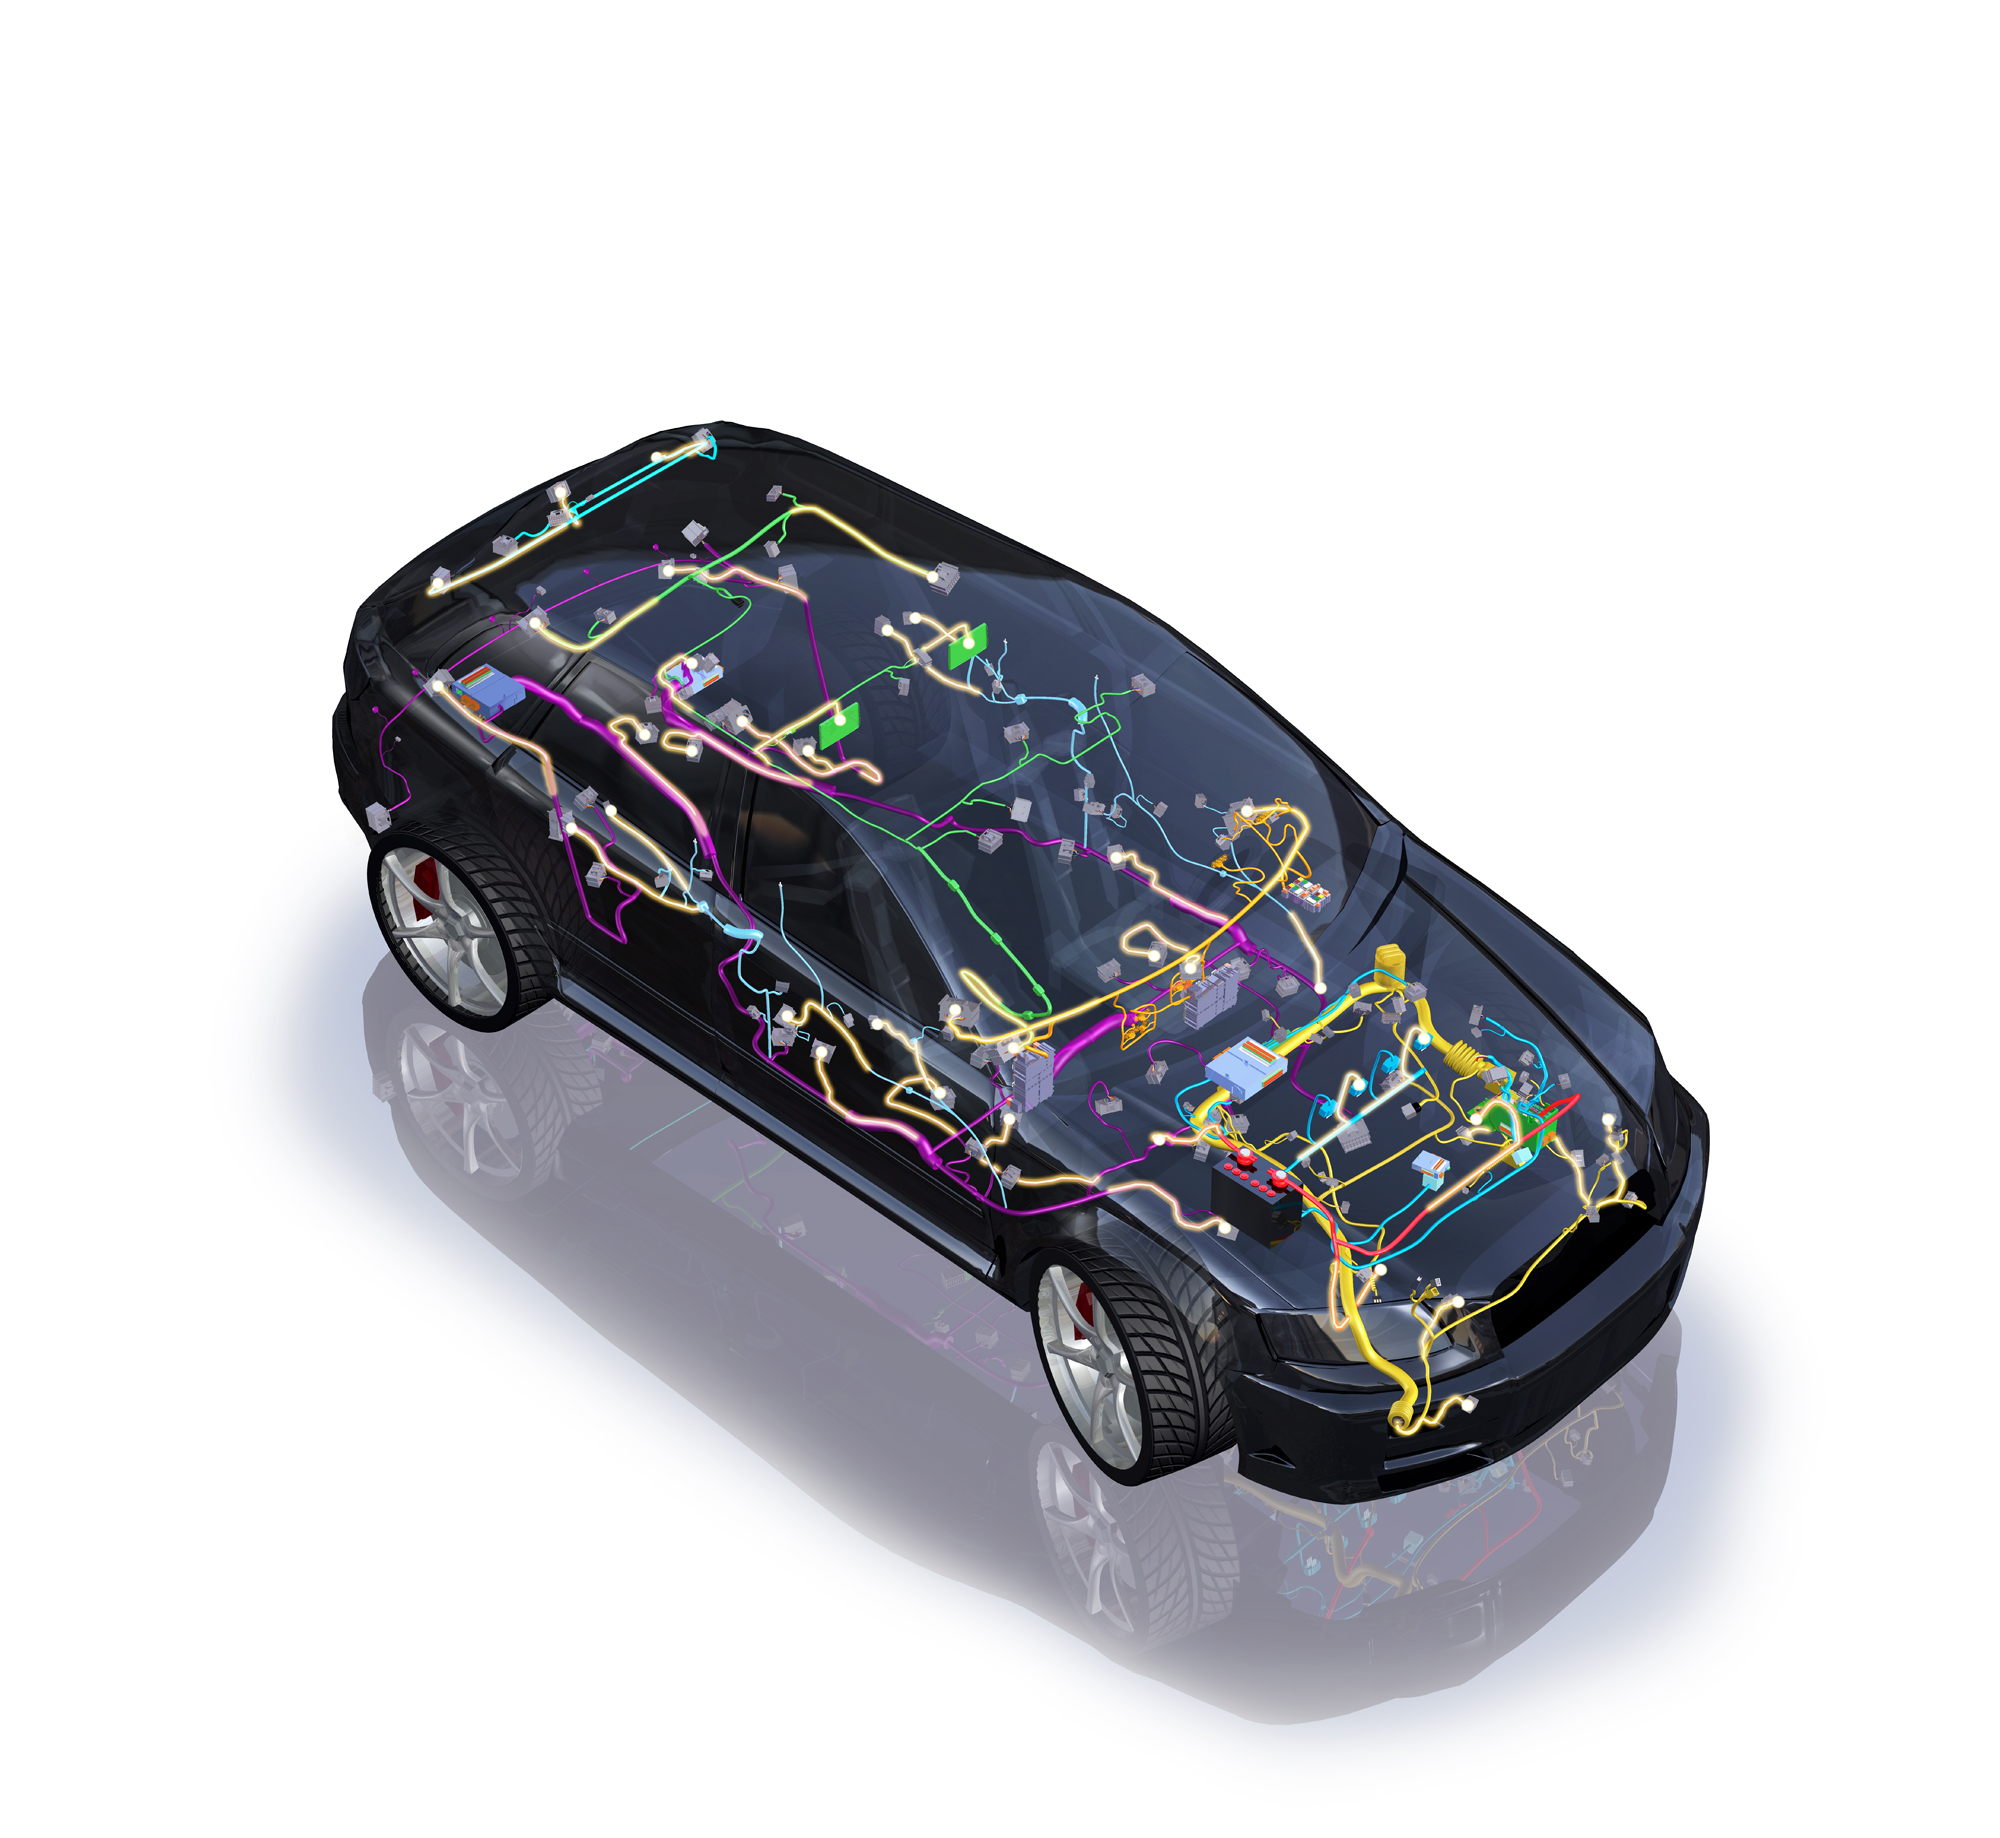
\includegraphics[width=0.7\linewidth]{figure/cover.jpg}
\end{figure}

% Cover text
\mbox{}
\vfill
\renewcommand{\familydefault}{\sfdefault} \normalfont % Set cover page font
\textbf{{\Huge
Improving the visualization of \\[0.2cm] 
electrical architectural diagrams}} \\[0.5cm]
{\normalfont
For different stakeholders using software metrics and data from Elektra} \\[0.5cm]
Master's thesis in Software Engineering \setlength{\parskip}{1cm}

{\large FLORENCE MAYO} \\[0.2cm]
{\large NATTAPON THATHONG} \setlength{\parskip}{1.5cm}

Department of Computer Science and Engineering \\
\textsc{Chalmers University of Technology} \\
\textsc{University of Gothenburg} \\
Gothenburg, Sweden 2016

\renewcommand{\familydefault}{\rmdefault} \normalfont % Reset standard font
\end{titlepage}


% BACK OF COVER PAGE (BLANK PAGE)
%\newpage
%\restoregeometry
%\thispagestyle{empty}
%\mbox{}


% TITLE PAGE
%\newpage
%\thispagestyle{empty}
%\begin{center}
%	\textsc{\large Master's thesis 2016:NN}\\[4cm]		% Report number given by department 
%	\textbf{\Large Improving the visualization of \\ electrical architectural diagrams} \\[1cm]
%	{\large For different stakeholders using software metrics \\ and data from Elektra}\\[1cm]
%	{\large FLORENCE MAYO \\[0.2cm] NATTAPON THATHONG}
	
%	\vfill	
	% Logotype on titlepage	
%	\begin{figure}[H]
%	\centering
	% Remove the following line to remove the titlepage logotype
%	
\includegraphics[width=0.2\pdfpagewidth]{figure/auxiliary/logo_eng.pdf}~~
%	
\includegraphics[width=0.27\pdfpagewidth]{figure/auxiliary/logo_gu_eng.png}\\	
%	\end{figure}	\vspace{5mm}	
	
%	Department of Computer Science and Engineering \\
%	\emph{Division of Software Engineering}\\
%	\textsc{Chalmers University of Technology} \\
%	\textsc{University of Gothenburg} \\
%	Gothenburg, Sweden 2016 \\
%\end{center}


% IMPRINT PAGE (BACK OF TITLE PAGE)
\newpage
\thispagestyle{plain}
The Author grants to Chalmers University of Technology and University of Gothenburg the non-exclusive right to publish the Work electronically and in a noncommercial purpose make it accessible on the Internet. The Author warrants that he/she is the author to the Work, and warrants that the Work does not contain text, pictures or other material that violates copyright law.\\
The Author shall, when transferring the rights of the Work to a third party (for example a publisher or a company), acknowledge the third party about this agreement. If the Author has signed a copyright agreement with a third party regarding the Work, the
Author warrants hereby that he/she has obtained any necessary permission from this third party to let Chalmers University of Technology and University of Gothenburg store the Work electronically and make it accessible on the Internet.

\vspace*{3.5cm}
Improving the visualization of electrical architectural diagrams\\
For different stakeholders using software metrics and data from Elektra\\[0.2cm]
FLORENCE MAYO, \\
NATTAPON THATHONG \setlength{\parskip}{1cm}

\copyright ~ FLORENCE MAYO, JUNE 2016. \\
\copyright ~ NATTAPON THATHONG, JUNE 2016.\setlength{\parskip}{1cm}

Examiner: ERIC KNAUSS \\
Supervisor: MICHEL CHAUDRON, PATRIZIO PELLICCIONE, \\ TRUONG HO QUANG, ULF ELIASSON
\setlength{\parskip}{1cm}

Master's Thesis 2015:NN\\	% Report number given by department 
Department of Computer Science and Engineering\\
Division of Software Engineering\\
Chalmers University of Technology and University of Gothenburg\\
SE-412 96 Gothenburg\\
Telephone +46 31 772 1000 \setlength{\parskip}{0.5cm}

\vfill
% Caption for cover page figure if used, possibly with reference to further information in the report
Cover: blah blah blah ... \todo{[to be filled in]} \setlength{\parskip}{0.5cm}

Typeset in \LaTeX \\
%Printed by [Name of printing company] \todo{[to be filled in]}\\
Gothenburg, Sweden 2016

